\chapter{Casi d'uso}

\section{UC1 - Inizializzazione del sistema}
\begin{figure}[h]
  \centering
  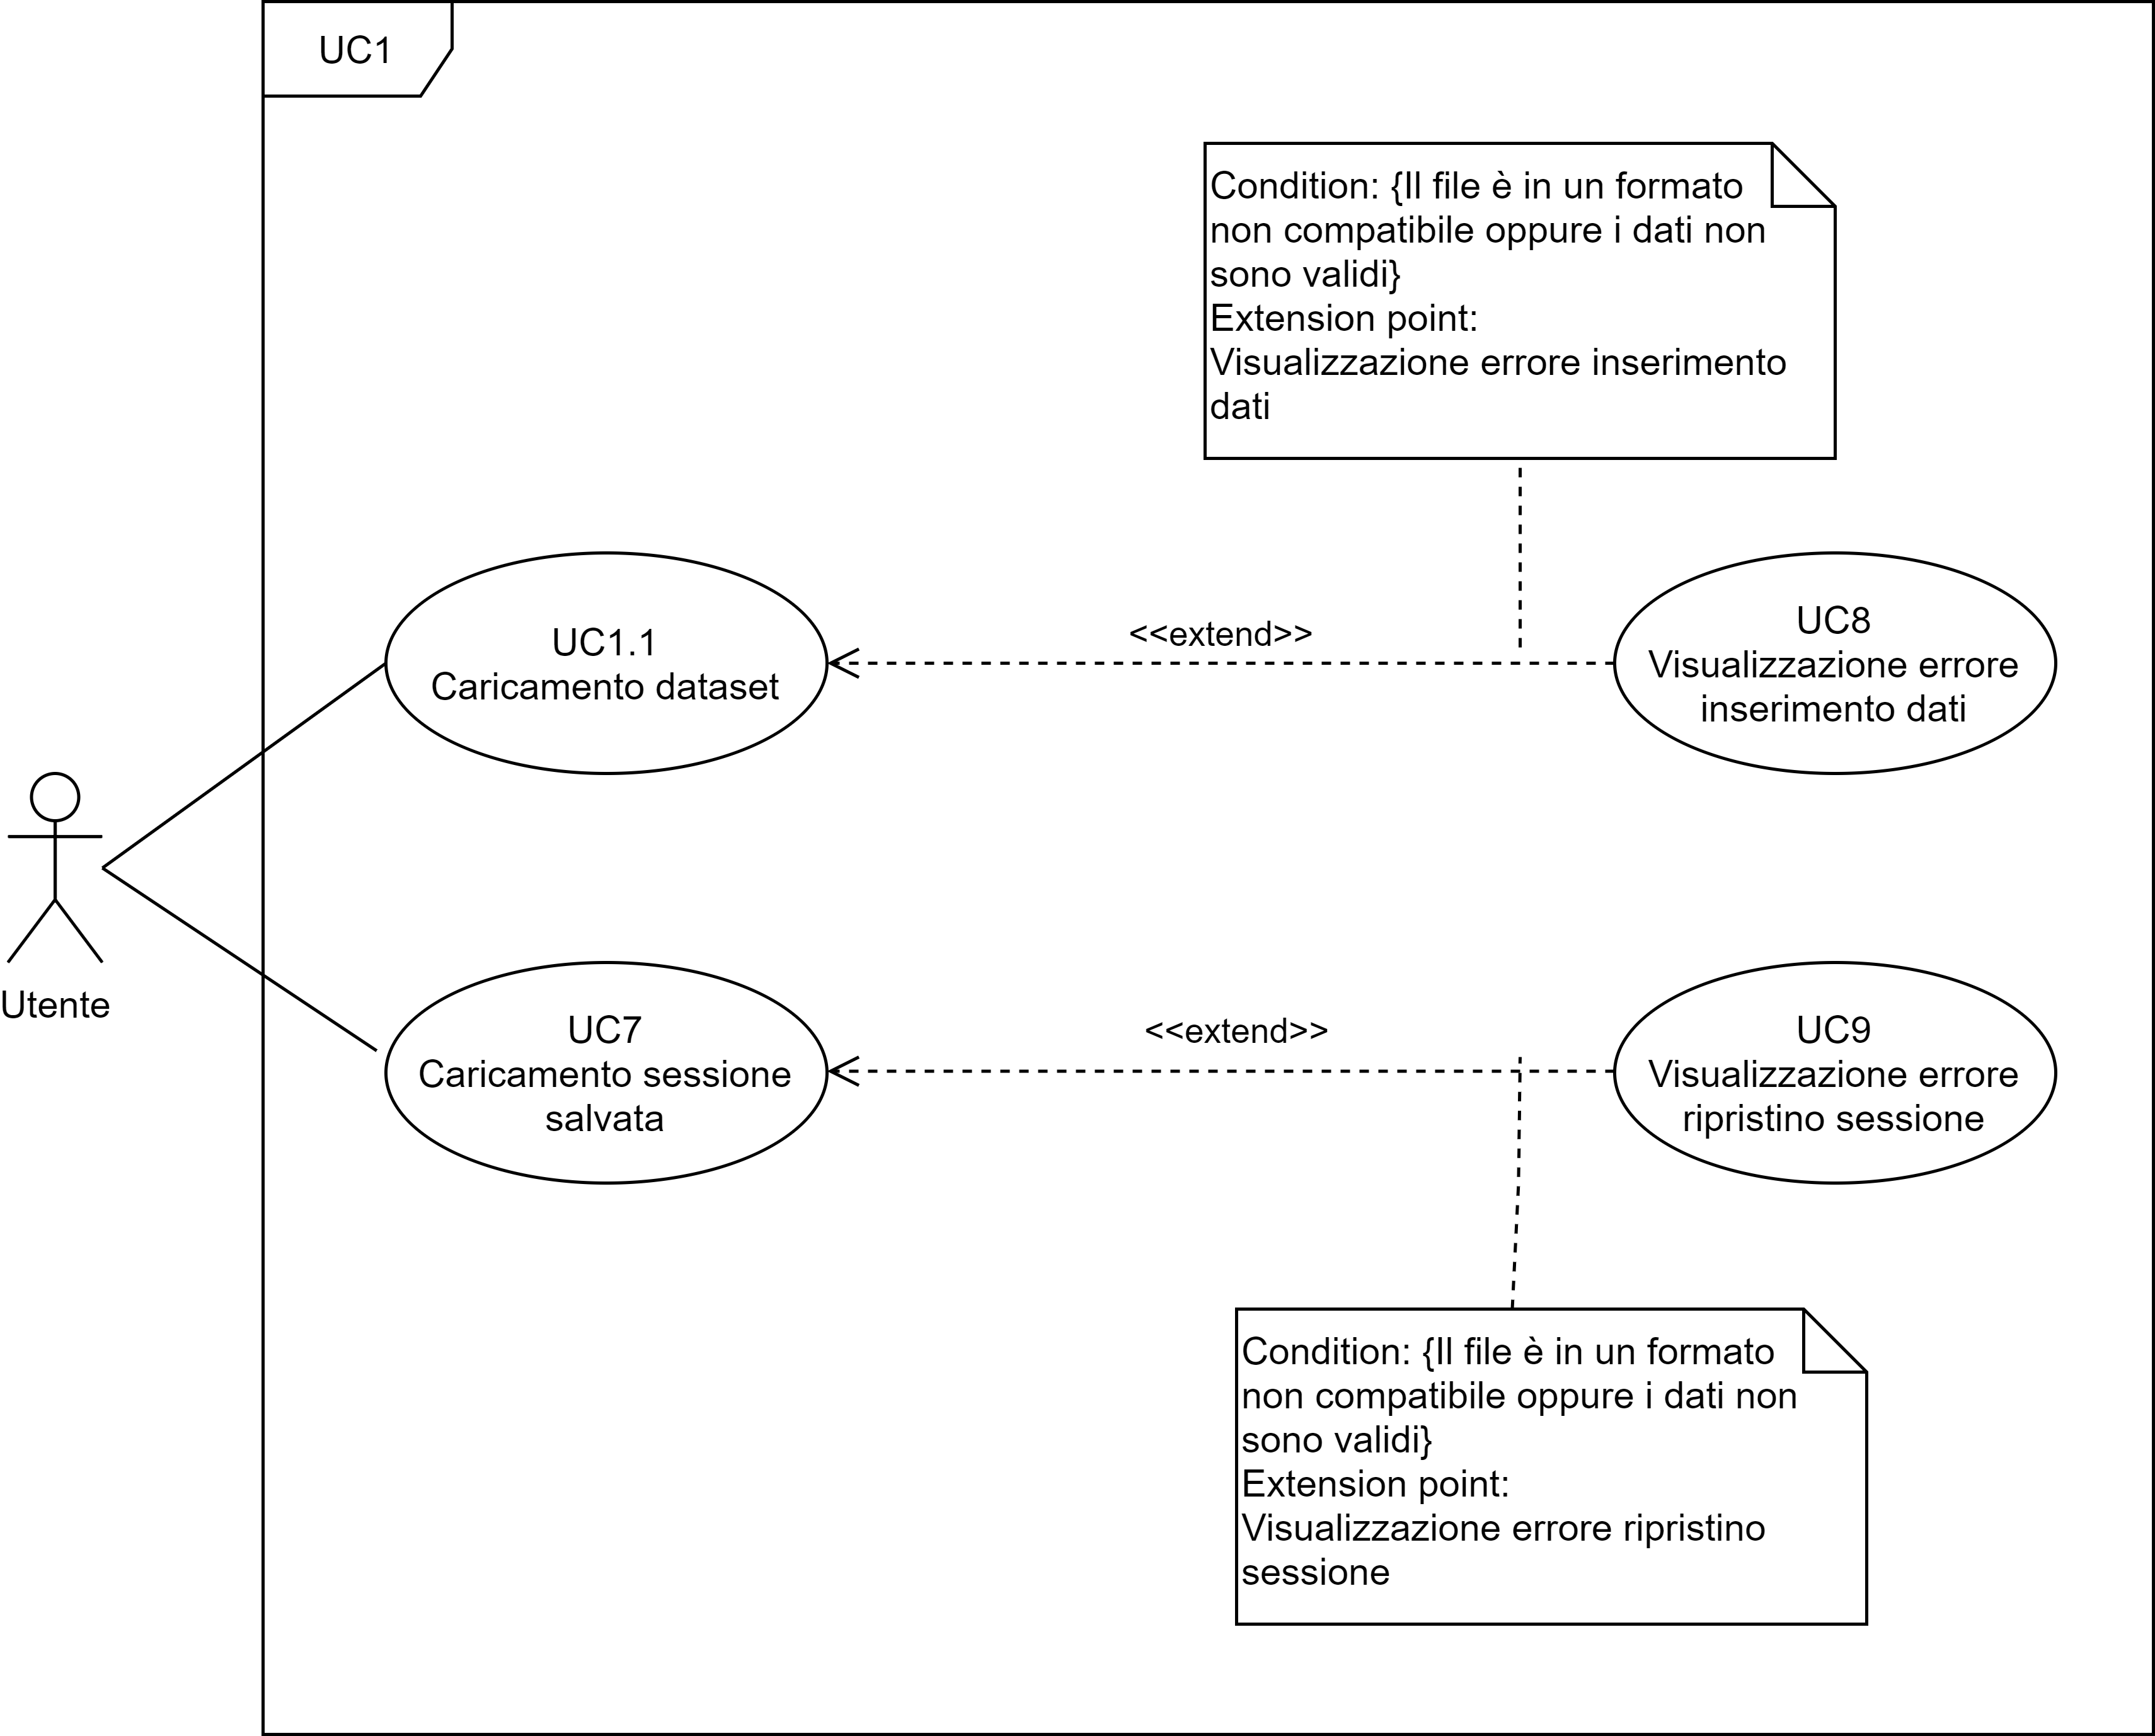
\includegraphics[width=0.6\textwidth]{UC1}
  \caption{UC1 - Inizializzazione del sistema}
\end{figure}
\begin{itemize}
     \item \textbf{Attore primario:} Utente.
     \item \textbf{Precondizioni:} Il sistema è raggiungibile e funzionante.
     \item \textbf{Postcondizioni:} Viene visualizzato un messaggio che indica il corretto caricamento dei dati. Questi dati sono disponibili per l'analisi.
     \item \textbf{Scenario principale:}
     \begin{enumerate}
       \item L'utente accede al sistema;
       \item L'utente carica un dataset [UC1.1];
       \item L'utente in alternativa può caricare una sessione precedentemente salvata [UC7].
     \end{enumerate}
     \item \textbf{Estensioni:}
     \begin{enumerate}
       \item Nel caso in cui il file sia in un formato non valido o i dati non siano validi:
       \begin{enumerate}
         \item Il caricamento non va a buon fine;
         \item Viene visualizzato un errore esplicativo [\todo{UC da mettere}].
       \end{enumerate}
       \item Nel caso in cui una sessione precedentemente salvata non sia ben formattata:
       \begin{enumerate}
         \item Il caricamento non va a buon fine;
         \item Viene visualizzato un errore esplicativo [\todo{UC da mettere}].
       \end{enumerate}
     \end{enumerate}
\end{itemize}
\subsection{UC1.1 - Caricamento dataset}
\begin{itemize}
  \item \textbf{Attore primario:} Utente.
  \item \textbf{Precondizioni:} Il sistema è raggiungibile e funzionante. L’utente ha a disposizione un dataset in formato CSV.
  \item \textbf{Postcondizioni:} I dati presenti nel file vengono caricati nel sistema. Viene visualizzato un messaggio che indica il corretto caricamento dei dati.
  \item \textbf{Scenario principale:} L'utente sceglie di caricare un dataset \todo{solo da locale? o anche da fonti esterne?}
\end{itemize}
\section{UC2}

\section{UC3}

\section{UC4}

\section{UC5}

\section{UC6}

\section{UC7}
